% Phase 2 presentation. Build:  cd presentation && tectonic slides.tex
\documentclass[aspectratio=169,11pt]{beamer}
\usepackage{tikz}
\usetikzlibrary{positioning,arrows.meta,fit,calc,shapes.geometric}
\usepackage{booktabs}
\usepackage{amsmath,amssymb}
\graphicspath{{../results/figures/}}

% ---------------------------------------------------------------- look
\definecolor{ink}{HTML}{1F1F1D}
\definecolor{ink2}{HTML}{52514E}
\definecolor{muted}{HTML}{898781}
\definecolor{rule}{HTML}{E1E0D9}
\definecolor{accent}{HTML}{2A78D6}
\definecolor{orange}{HTML}{EB6834}
\definecolor{green}{HTML}{1BAF7A}
\definecolor{violet}{HTML}{6250D6}
\definecolor{paper}{HTML}{FCFCFB}
\setbeamercolor{background canvas}{bg=paper}
\setbeamercolor{normal text}{fg=ink}
\setbeamercolor{frametitle}{fg=ink,bg=paper}
\setbeamercolor{title}{fg=ink}
\setbeamercolor{subtitle}{fg=ink2}
\setbeamercolor{structure}{fg=accent}
\setbeamercolor{itemize item}{fg=accent}
\setbeamercolor{block title}{fg=paper,bg=accent}
\setbeamercolor{block body}{bg=rule!40}
\setbeamerfont{frametitle}{size=\Large,series=\bfseries}
\setbeamertemplate{navigation symbols}{}
\setbeamertemplate{itemize items}{\raisebox{0.15ex}{\scriptsize$\blacksquare$}}
\setbeamertemplate{footline}{%
  \hspace{1em}{\color{muted}\scriptsize Traffic flow prediction on METR-LA \textperiodcentered{} Phase 2}%
  \hfill{\color{muted}\scriptsize\insertframenumber/\inserttotalframenumber}\hspace{1em}\vspace{0.6em}}
\setbeamertemplate{frametitle}{\vspace{0.4em}\insertframetitle\par\vspace{-0.2em}%
  {\color{accent}\rule{2.2em}{2pt}}}
\newcommand{\kicker}[1]{{\color{accent}\scriptsize\bfseries\MakeUppercase{#1}}\par\vspace{0.3em}}
\newcommand{\hl}[1]{{\color{accent}\bfseries #1}}
\newcommand{\aside}[1]{{\color{muted}\footnotesize #1}}
\tikzset{
  box/.style={draw=ink2, rounded corners=2pt, fill=white, minimum height=2.2em, align=center, font=\footnotesize, inner sep=4pt},
  dl/.style={box, draw=accent, fill=accent!8},
  ml/.style={box, draw=orange, fill=orange!8},
  arr/.style={-{Stealth[length=2mm]}, thick, ink2},
}

% TODO: replace with your names and institution
\title{Traffic Flow Prediction and Simulated Signal Control}
\subtitle{From independent segment models to a graph attention hybrid on METR-LA}
\author{Student Name 1, Student Name 2}
\institute{Applied Machine Learning \textperiodcentered{} Phase 2: Deep Learning and Hybrid}
\date{}

\begin{document}

\begin{frame}[plain]
\titlepage
\end{frame}

% ================================================================ problem
\begin{frame}{The question}
\kicker{Project brief}
\begin{columns}[T]
\column{0.55\textwidth}
\begin{itemize}\setlength\itemsep{0.6em}
\item Forecast freeway \hl{speed} at 207 LA sensors, 5--60 min ahead (METR-LA, Mar--Jun 2012, 5-min data).
\item \textbf{Does network-aware graph learning beat independent per-segment models?} And where?
\item Simulate (never claim) a congestion-responsive signal policy.
\end{itemize}
\column{0.42\textwidth}
\begin{block}{The hybrid logic}
\footnotesize
\textbf{AML baseline:} one XGBoost per road segment, own lags + calendar.\\[0.3em]
\textbf{Gap:} it cannot see congestion propagating along the road.\\[0.3em]
\textbf{DL:} graph attention over the fixed road graph.\\[0.3em]
\textbf{Hybrid:} GAT learns the network correction to XGBoost.
\end{block}
\end{columns}
\end{frame}

\begin{frame}{Data and a fair protocol}
\kicker{Dataset construction}
\begin{columns}[T]
\column{0.5\textwidth}
\begin{itemize}\setlength\itemsep{0.45em}
\item 34,272 steps $\times$ 207 sensors; \hl{8\,\%} readings missing (stored as 0 mph).
\item Road graph: Gaussian kernel on road distance, \hl{1,515} directed edges, 73\,\% one-way, median edge 2.8\,km (NetworkX).
\item Chronological 70/10/20 split, \hl{never shuffled} across boundaries.
\item Every model: same \hl{12-step (1 h)} history, same 12 horizons, same anchors.
\end{itemize}
\column{0.47\textwidth}
\begin{itemize}\setlength\itemsep{0.45em}
\item Scaler, weekly profile, XGBoost: fitted on \hl{training} timestamps only.
\item Outages \hl{masked}, not zero traffic: forward-fill + 0/1 mask channel; missing targets excluded from loss and metrics.
\item \hl{Cyclic time}: sin/cos of time of day and day of week.
\item Metrics: MAE, RMSE, MAPE at \emph{every} horizon; peak vs off-peak; DM tests.
\end{itemize}
\end{columns}
\end{frame}

% ================================================================ baseline + gap
\begin{frame}{AML baseline: XGBoost per segment}
\kicker{207 independent models}
\begin{columns}[T]
\column{0.52\textwidth}
\begin{itemize}\setlength\itemsep{0.45em}
\item One \hl{multi-output} XGBoost per sensor (vector-leaf trees predict all 12 horizons), absolute-error loss, depth 6, early stopping.
\item 37 features of the sensor's \emph{own} series: 12 lags, differences, rolling mean/std/min, missing count, sin/cos time, weekday, weekly profile at the 12 target times, anomaly.
\item No other sensor enters, \hl{by design}.
\end{itemize}
\column{0.45\textwidth}
\begin{block}{Why speed only?}
\footnotesize METR-LA publishes speed only; flow and occupancy would need raw PeMS station files (future extension).
\end{block}
\vspace{0.5em}
\begin{block}{Leakage-free base forecasts}
\footnotesize Training-period forecasts are \textbf{out-of-fold}: 5 contiguous blocks, 23-step purge so no window overlaps the held-out block.
\end{block}
\end{columns}
\end{frame}

\begin{frame}{The gap, measured before any deep model}
\kicker{Out-of-fold training residuals only; no test data}
\centering
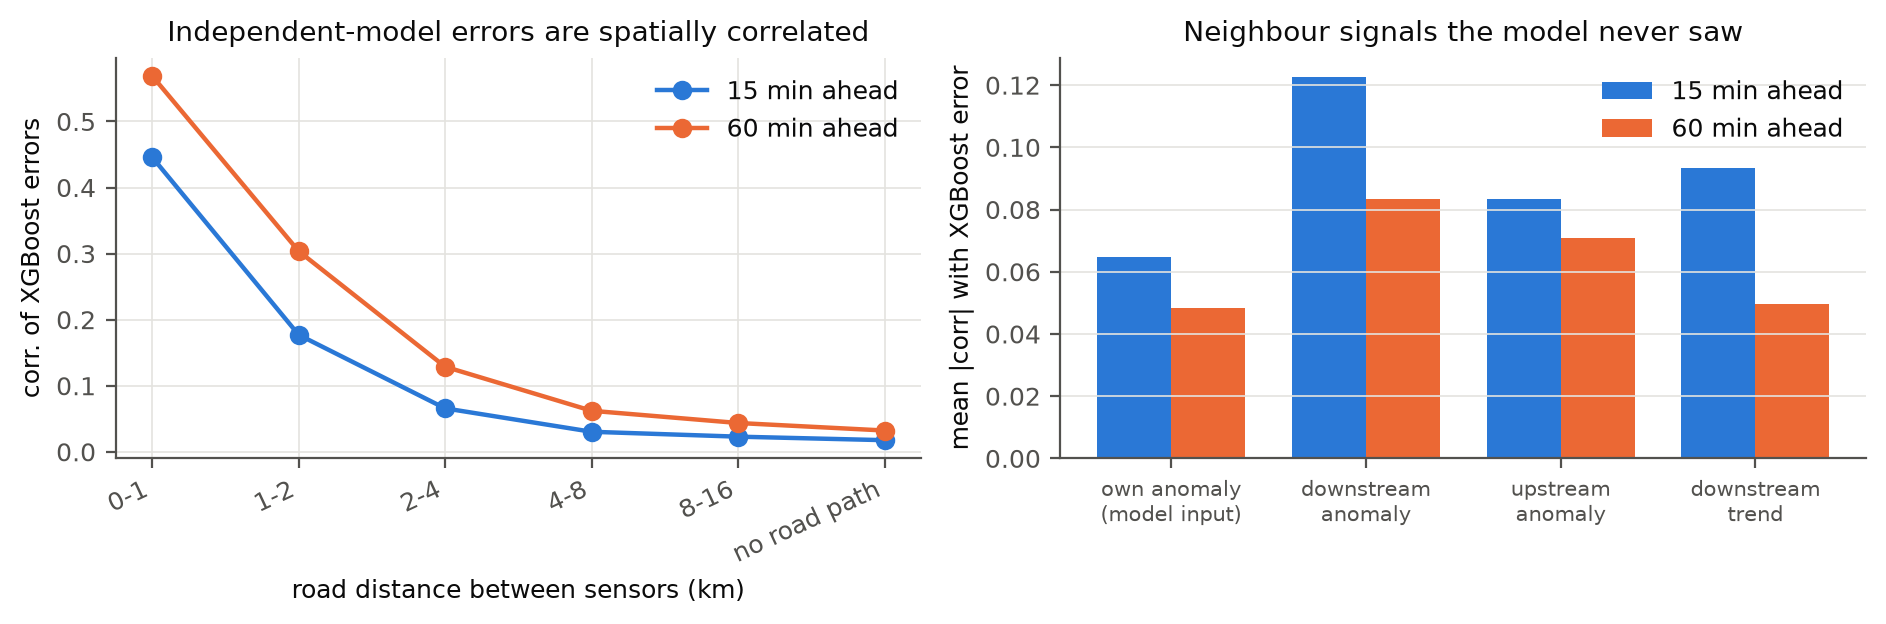
\includegraphics[width=0.92\textwidth]{p2_gap_analysis.png}\\[0.2em]
\small Best independent forecast loses
$\mathbb{E}\big[(\mathbb{E}[y\,|\,\text{network}]-\mathbb{E}[y\,|\,\text{own}])^2\big]\ge 0$:
errors of road neighbours correlate (\hl{0.21} vs 0.04 at 60 min), and the \emph{downstream} anomaly
predicts the error better than the sensor's own.
\end{frame}

% ================================================================ architecture
\begin{frame}{ST-GAT: spatio-temporal graph attention network}
\kicker{Architecture logic}
\centering
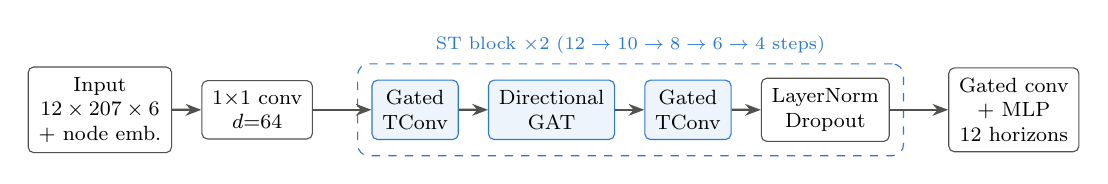
\begin{tikzpicture}[node distance=4mm and 4mm, scale=0.93, transform shape]
\node[box] (in) {Input\\$12\times207\times6$\\+ node emb.};
\node[box, right=of in] (lift) {$1{\times}1$ conv\\$d{=}64$};
\node[dl, right=8mm of lift] (t1) {Gated\\TConv};
\node[dl, right=of t1] (gat) {Directional\\GAT};
\node[dl, right=of gat] (t2) {Gated\\TConv};
\node[box, right=of t2] (ln) {LayerNorm\\Dropout};
\node[draw=accent, dashed, rounded corners, fit=(t1)(gat)(t2)(ln), inner sep=5pt,
      label={[font=\scriptsize, text=accent]above:ST block $\times 2$ ($12\to10\to8\to6\to4$ steps)}] (blk) {};
\node[box, right=8mm of ln] (out) {Gated conv\\+ MLP\\12 horizons};
\draw[arr] (in) -- (lift); \draw[arr] (lift) -- (t1); \draw[arr] (t1) -- (gat);
\draw[arr] (gat) -- (t2); \draw[arr] (t2) -- (ln); \draw[arr] (ln) -- (out);
\end{tikzpicture}
\vspace{1em}
\begin{columns}[T]
\column{0.48\textwidth}
\begin{itemize}\setlength\itemsep{0.35em}\small
\item Gated temporal conv (STGCN): $\Gamma(H)=(P+H)\odot\sigma(Q)$.
\item Attention on the \hl{fixed road graph}, separately over \hl{downstream} and \hl{upstream} neighbours (queues spill back upstream).
\end{itemize}
\column{0.48\textwidth}
\begin{itemize}\setlength\itemsep{0.35em}\small
\item 164k parameters.
\item Receptive field: all 12 steps; 2 hops each way ($\approx$36 sensors).
\item Masked MAE loss in mph (median-optimal, robust to congestion tail).
\end{itemize}
\end{columns}
\end{frame}

\begin{frame}{Graph attention: why, and how it differs}
\kicker{Theoretical rigour}
\begin{columns}[T]
\column{0.55\textwidth}
\small
\[
\alpha_{ij}=\operatorname{softmax}_{j\in\mathcal{N}(i)}\operatorname{LeakyReLU}\big(\mathbf{a}_{\mathrm{dst}}^{\top}W\bar h_i+\mathbf{a}_{\mathrm{src}}^{\top}W\bar h_j\big)
\]
\[
h'_{t,i}=\big\Vert_{k=1}^{K}\textstyle\sum_{j\in\mathcal{N}(i)}\alpha^{k}_{ij}W^{k}h_{t,j}
\]
\begin{itemize}\setlength\itemsep{0.35em}\small
\item Diffusion conv: weights fixed by distance. GAT: weights depend on the \hl{current state}.
\item $\mathbf{a}=\mathbf{0}$ gives the mean aggregator, so attention \hl{strictly generalises} it.
\end{itemize}
\column{0.42\textwidth}
\begin{itemize}\setlength\itemsep{0.35em}\small
\item Coefficients from the window-averaged state $\bar h$, shared by its 12 steps (as ASTGCN): one masked $N{\times}N$ product per head, $T{=}12\times$ fewer attention scores.
\item With $T{=}1$ it \hl{equals} PyG \texttt{GATConv} (unit test, $10^{-5}$).
\item Only the node embedding breaks permutation equivariance, deliberately.
\end{itemize}
\end{columns}
\end{frame}

\begin{frame}{Hybrid: XGBoost per segment $\to$ graph attention}
\kicker{Hybrid innovation}
\centering
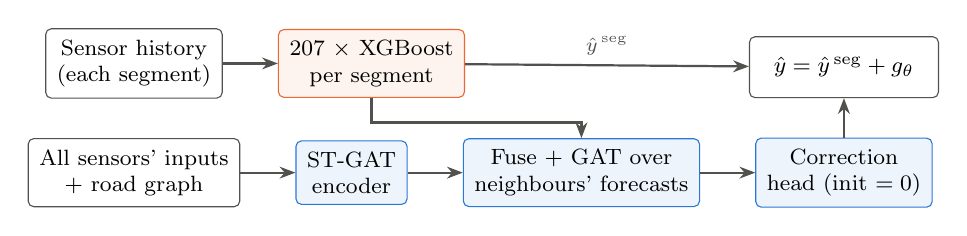
\begin{tikzpicture}[node distance=5mm and 7mm]
\node[box] (x) {Sensor history\\(each segment)};
\node[ml, right=of x] (xgb) {207 $\times$ XGBoost\\per segment};
\node[box, below=of x] (g) {All sensors' inputs\\+ road graph};
\node[dl, right=of g] (st) {ST-GAT\\encoder};
\node[dl, right=of st] (fuse) {Fuse + GAT over\\neighbours' forecasts};
\node[dl, right=of fuse] (head) {Correction\\head (init $=0$)};
\node[box, above=5mm of head, minimum width=2.4cm] (sum) {$\hat y=\hat y^{\,\mathrm{seg}}+g_\theta$};
\draw[arr] (x) -- (xgb); \draw[arr] (g) -- (st); \draw[arr] (st) -- (fuse); \draw[arr] (fuse) -- (head);
\draw[arr] (xgb) -- node[above, font=\scriptsize]{$\hat y^{\,\mathrm{seg}}$} (sum);
\draw[arr] (xgb.south) |- ([yshift=2mm]fuse.north) -- (fuse.north);
\draw[arr] (head) -- (sum);
\end{tikzpicture}
\vspace{0.8em}
\begin{columns}[T]
\column{0.5\textwidth}
\begin{itemize}\setlength\itemsep{0.35em}\small
\item Trees do the per-segment job (level, seasonality, thresholds); GAT does what trees \hl{structurally cannot}: cross-segment propagation.
\item Zero-initialised head: training \hl{starts exactly at XGBoost} (unit test).
\end{itemize}
\column{0.47\textwidth}
\begin{itemize}\setlength\itemsep{0.35em}\small
\item \hl{Cross-fitting}: GAT trains on out-of-fold XGBoost forecasts, so it sees realistic errors (in-sample MAE 2.69 vs 2.99 out-of-fold).
\item Precedent: residual hybrids (Zhang 2003), stacking (Wolpert 1992).
\end{itemize}
\end{columns}
\end{frame}

\begin{frame}{Deep learning dataset and regularisation}
\kicker{164k parameters, 24k strongly overlapping windows}
\begin{columns}[T]
\column{0.5\textwidth}
\begin{itemize}\setlength\itemsep{0.45em}\small
\item Sliding 24-step windows (12 in, 12 out) by anchor time.
\item Dropout 0.2; attention dropout 0.1 (DropEdge-like).
\item LayerNorm; AdamW, weight decay $10^{-4}$.
\item Gradient clipping at norm 5.
\end{itemize}
\column{0.47\textwidth}
\begin{itemize}\setlength\itemsep{0.45em}\small
\item LR halved after 3 flat epochs; early stopping, patience 8; best-validation checkpoint.
\item Each epoch: a fresh random \hl{half} of training windows (adjacent windows share 11/12 steps).
\item Small node embeddings (16-d). One seed (0) per configuration.
\end{itemize}
\end{columns}
\vspace{0.6em}
\centering
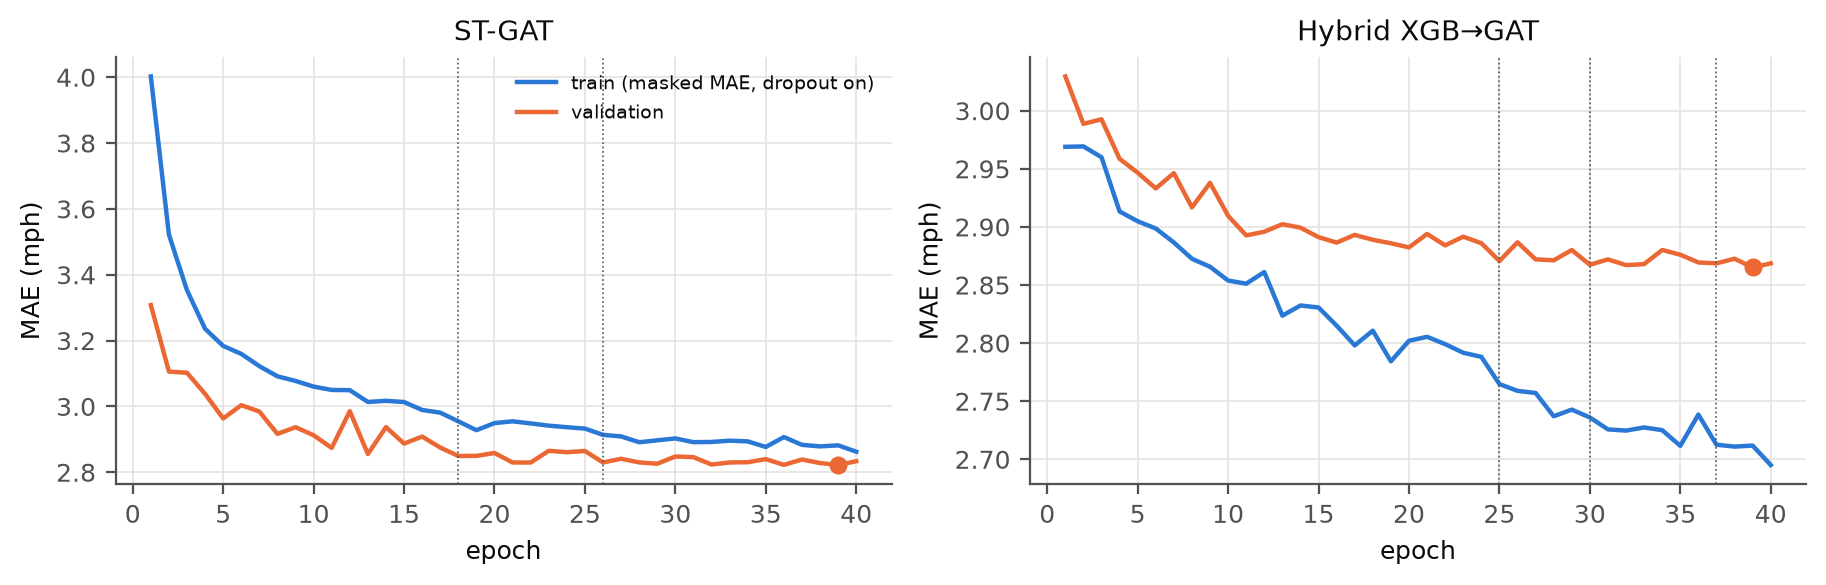
\includegraphics[height=0.27\textheight]{p2_learning_curves.png}
\end{frame}

% ================================================================ results
\begin{frame}{Results: network-aware models win}
\kicker{Test MAE (mph), 4--27 June 2012, same 1-hour history for every model}
\begin{columns}[T]
\column{0.56\textwidth}
\footnotesize\setlength{\tabcolsep}{4pt}
\begin{tabular}{lcccc}
\toprule
Model & 15 & 30 & 60 & avg \\
\midrule
Historical average & 4.19 & 4.19 & 4.19 & 4.19 \\
Gradient boosting (features) & 2.89 & 3.29 & 3.66 & 3.22 \\
\textcolor{orange}{XGBoost per segment} & 2.89 & 3.26 & 3.64 & 3.20 \\
\textcolor{accent}{ST-GAT (ours)} & 2.74 & \textbf{3.08} & \textbf{3.47} & \textbf{3.04} \\
\textcolor{green}{Hybrid XGB$\to$GAT (ours)} & \textbf{2.72} & 3.09 & 3.52 & 3.06 \\
\bottomrule
\end{tabular}
\column{0.41\textwidth}
\begin{itemize}\setlength\itemsep{0.4em}\small
\item ST-GAT: \hl{$-5\,\%$} vs.\ per-segment XGBoost; hybrid $-4.5\,\%$.
\item Diebold--Mariano vs.\ XGBoost: \hl{$p<0.001$} at 15, 30, 60 min.
\item Hybrid best at 15 min; ST-GAT best at 30/60 min after long training.
\item ST-GAT 3.47 at 60 min: below published DCRNN (3.60) and Graph WaveNet (3.53).
\end{itemize}
\end{columns}
\end{frame}

\begin{frame}{Accuracy at every horizon}
\kicker{Fair comparison}
\centering
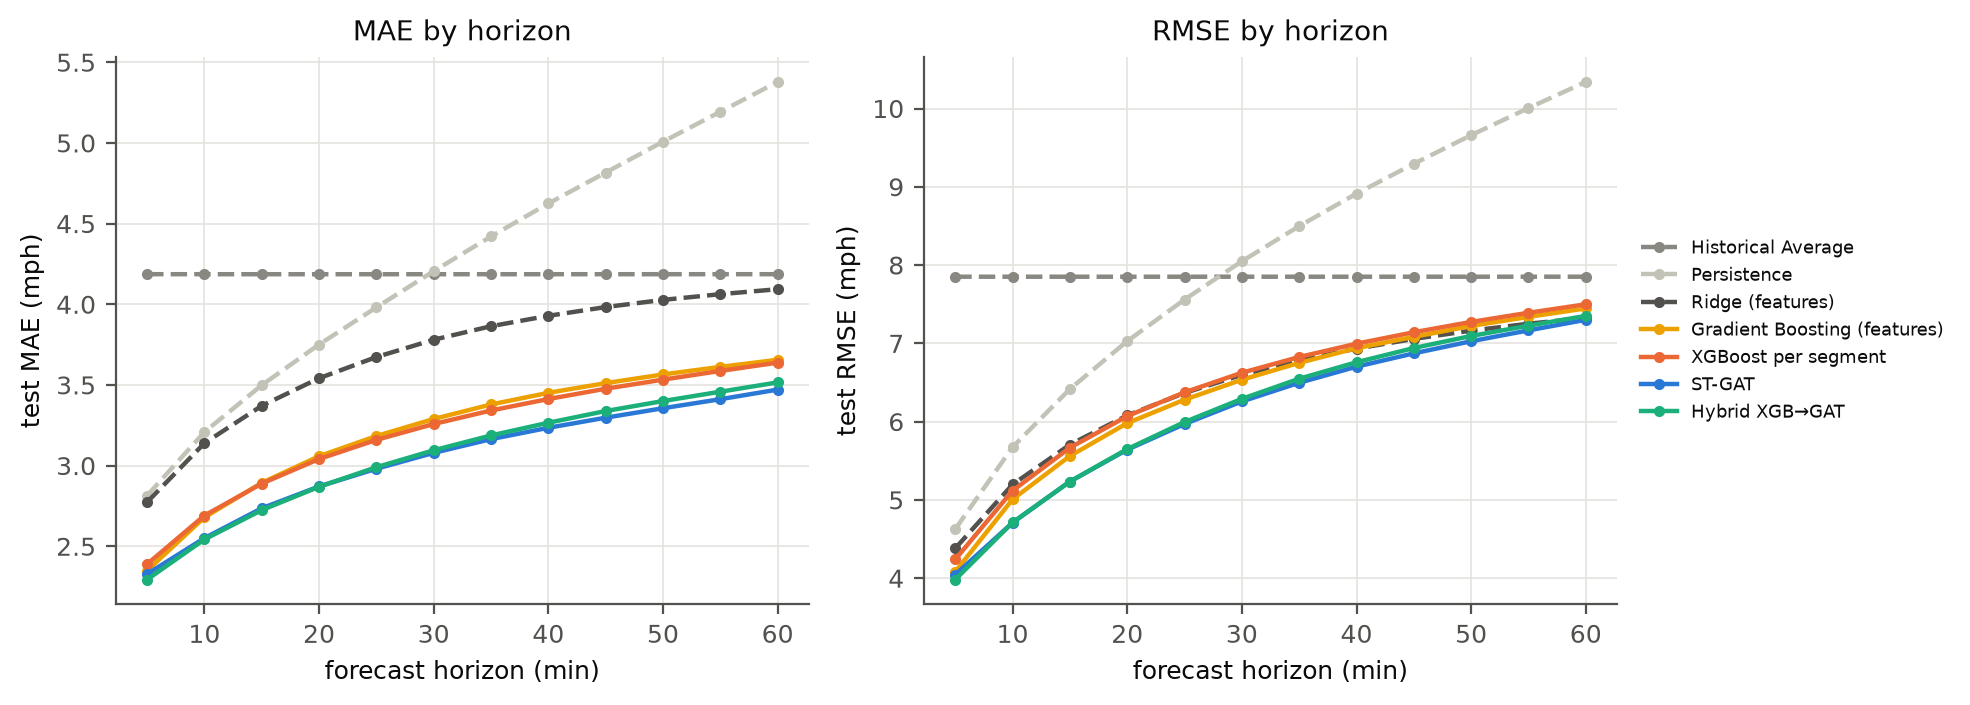
\includegraphics[width=0.92\textwidth]{p2_horizon_metrics.png}\\[0.3em]
\aside{MAE and RMSE at all 12 horizons (5--60 min). Dashed: simple baselines.}
\end{frame}

\begin{frame}{Peak, off-peak and congestion}
\kicker{Peak = weekdays 06--10 and 15--19 (by target time)}
\centering
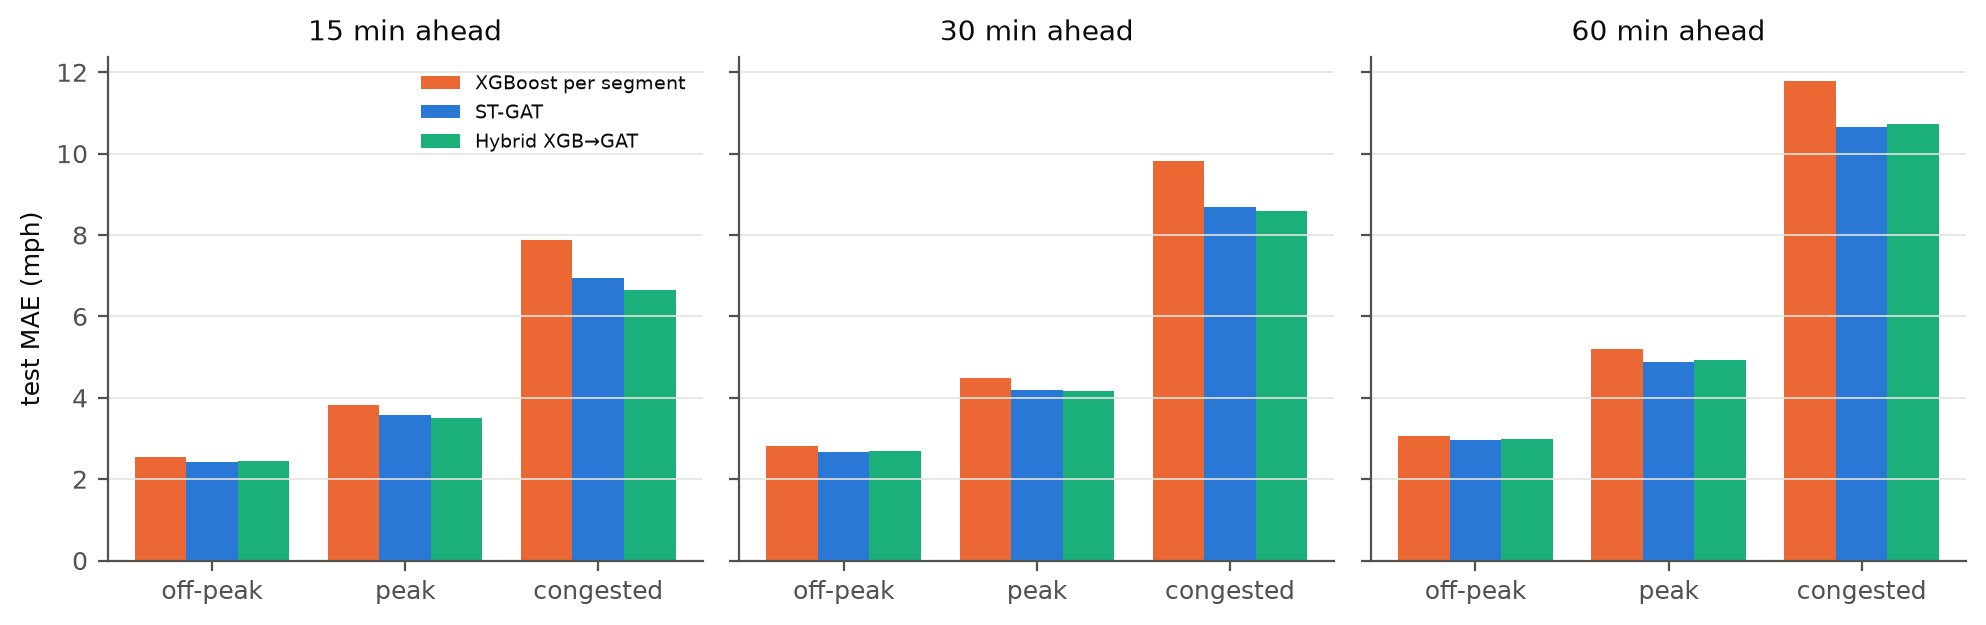
\includegraphics[width=0.95\textwidth]{p2_peak_offpeak.png}\\[0.4em]
\small Peak, 60 min: XGBoost 5.19 $\to$ \hl{ST-GAT 4.88 mph ($-6\,\%$)}; off-peak 3.07 $\to$ 2.96 ($-3.6\,\%$).
Congested targets ($<$40 mph): both network models cut the error by more than 1 mph (11.79 $\to$ 10.66 / 10.74).
\end{frame}

\begin{frame}{Congestion map: forecasts made 60 minutes earlier}
\kicker{Deliverable}
\centering
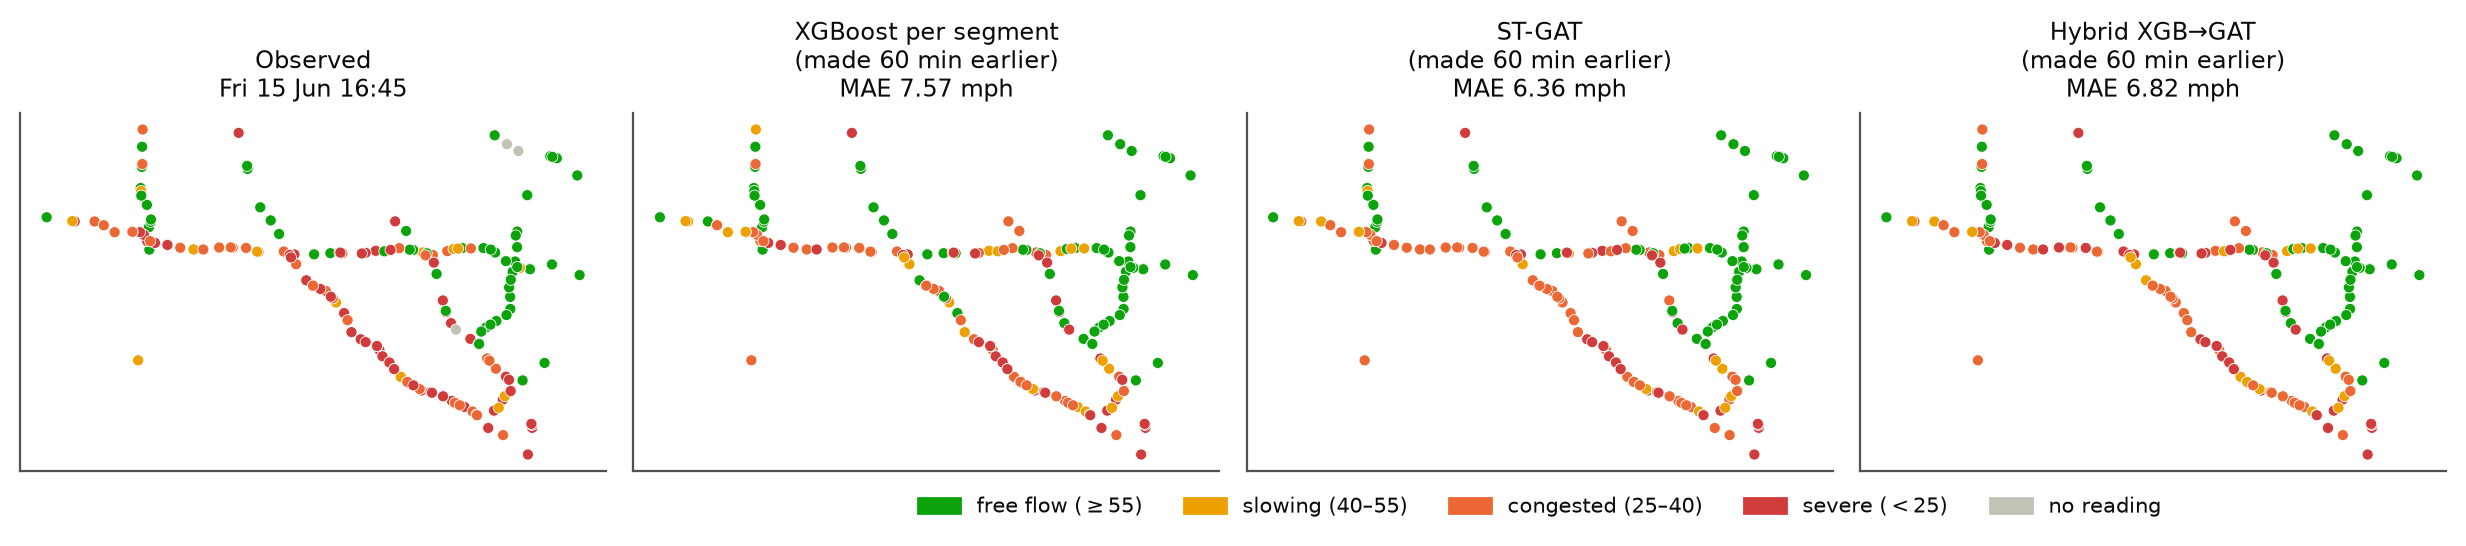
\includegraphics[width=\textwidth]{p2_congestion_map.png}\\[0.5em]
\begin{columns}[T]
\column{0.48\textwidth}
\centering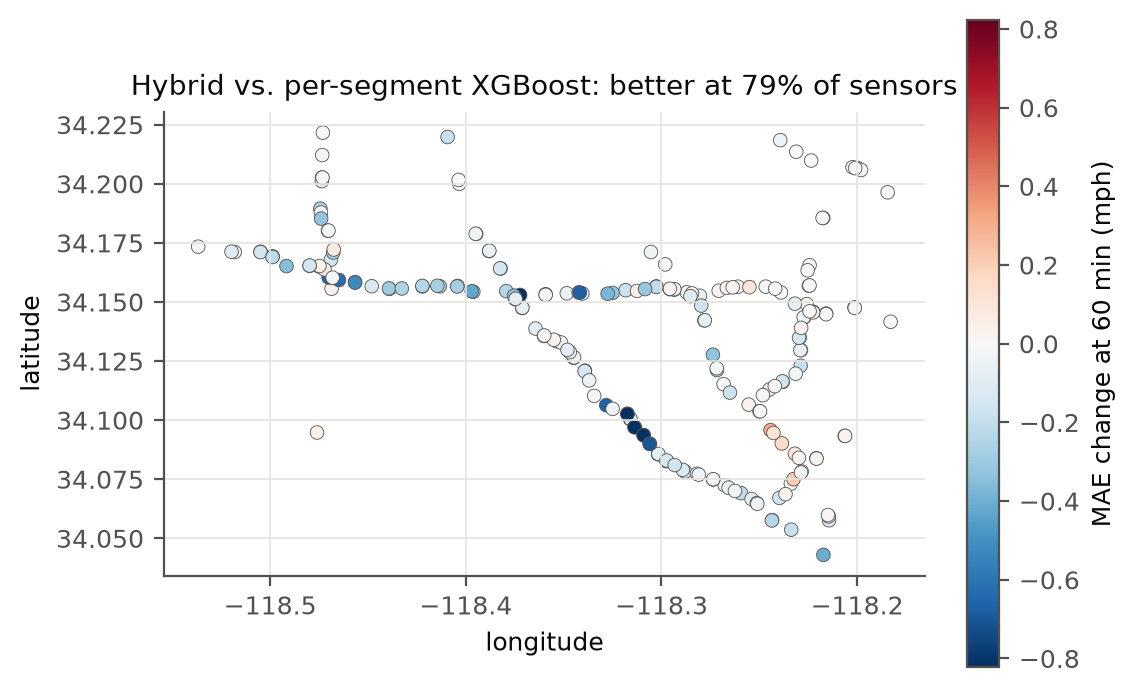
\includegraphics[height=0.36\textheight]{p2_improvement_map.png}
\column{0.48\textwidth}
\small
\begin{itemize}\setlength\itemsep{0.4em}
\item The independent model misses how far the evening slowdown spreads.
\item Hybrid beats XGBoost at \hl{79\,\%} of sensors at 60 min, most along the congested corridor.
\end{itemize}
\end{columns}
\end{frame}

\begin{frame}{Ablation: what is each part of ST-GAT worth?}
\kicker{Ablation studies \textperiodcentered{} same 12-epoch budget, same seed; test MAE (mph)}
\begin{columns}[T]
\column{0.58\textwidth}
\footnotesize\setlength{\tabcolsep}{3.5pt}
\begin{tabular}{lcccc}
\toprule
ST-GAT variant & 15 & 30 & 60 & avg \\
\midrule
\textcolor{accent}{Full (road-graph attention, masked)} & \textbf{2.76} & \textbf{3.12} & \textbf{3.53} & \textbf{3.08} \\
Mean aggregation (no attention) & 2.76 & 3.14 & 3.55 & 3.10 \\
Attention over all pairs (no road prior) & 2.83 & 3.19 & 3.56 & 3.14 \\
No spatial module & 2.86 & 3.25 & 3.71 & 3.20 \\
Outages fed as 0 mph (no mask) & 2.84 & 3.26 & 3.79 & 3.23 \\
\bottomrule
\end{tabular}
\column{0.39\textwidth}
\begin{itemize}\setlength\itemsep{0.35em}\small
\item \hl{Outage masking} matters most: +0.26 at 60 min without it.
\item \hl{No graph} $\Rightarrow$ 3.20, exactly per-segment XGBoost: the gain is the network.
\item \hl{Road prior} beats attention over all pairs (+0.06).
\item Attention vs.\ plain averaging: only 0.02.
\end{itemize}
\end{columns}
\end{frame}

\begin{frame}{Ablation: why the hybrid is built this way}
\kicker{Hybrid innovation \textperiodcentered{} every variant corrects the same XGBoost forecasts}
\begin{columns}[T]
\column{0.58\textwidth}
\footnotesize\setlength{\tabcolsep}{3.5pt}
\begin{tabular}{lcccc}
\toprule
Hybrid variant & 15 & 30 & 60 & avg \\
\midrule
\textcolor{green}{Full (cross-fitted, residual, GAT)} & \textbf{2.73} & \textbf{3.08} & \textbf{3.50} & \textbf{3.05} \\
Base as input only (no residual) & 2.75 & 3.10 & 3.52 & 3.07 \\
In-sample base (no cross-fitting) & 2.82 & 3.20 & 3.58 & 3.14 \\
Correction without graph & 2.84 & 3.21 & 3.60 & 3.16 \\
Linear neighbour correction & 2.87 & 3.25 & 3.63 & 3.19 \\
XGBoost per segment alone & 2.89 & 3.26 & 3.64 & 3.20 \\
\bottomrule
\end{tabular}
\column{0.39\textwidth}
\begin{itemize}\setlength\itemsep{0.35em}\small
\item \hl{Graph} is essential: without it the correction barely helps.
\item \hl{Cross-fitting} is essential: in-sample bases lose most of the gain.
\item Residual connection: +0.02.
\item Same budget: hybrid beats ST-GAT at \hl{every horizon} (3.05 vs.\ 3.08).
\end{itemize}
\end{columns}
\end{frame}

\begin{frame}{Validation and robustness}
\kicker{Technical validation}
\begin{columns}[T]
\column{0.5\textwidth}
\begin{itemize}\setlength\itemsep{0.4em}\small
\item \hl{Diebold--Mariano} with Newey--West variance (overlapping windows are autocorrelated).
\item \hl{Day-block bootstrap} 95\,\% CIs: ST-GAT [2.85, 3.16], XGBoost [2.99, 3.35]; day-to-day variance is large, paired tests are decisive.
\item \hl{52 unit tests}: GAT = PyG \texttt{GATConv}, masks respected, no-graph independence, hybrid starts at XGBoost, causal features, fold purging, graph statistics.
\end{itemize}
\column{0.46\textwidth}
\small
\textbf{Latest reading missing} (60-min MAE change)\\[0.3em]
\begin{tabular}{lc}
\toprule
XGBoost per segment & +32\,\% \\
\textcolor{accent}{ST-GAT (masked)} & \textbf{+28\,\%} \\
Hybrid XGB$\to$GAT & +34\,\% \\
\bottomrule
\end{tabular}\\[0.6em]
\aside{Ablation: the same ST-GAT fed 0 mph for outages is 0.26 mph worse at 60 min. Same seed $\Rightarrow$ identical losses on re-run (reproducible).}
\end{columns}
\end{frame}

\begin{frame}{Where does ST-GAT look?}
\kicker{Attention analysis}
\centering
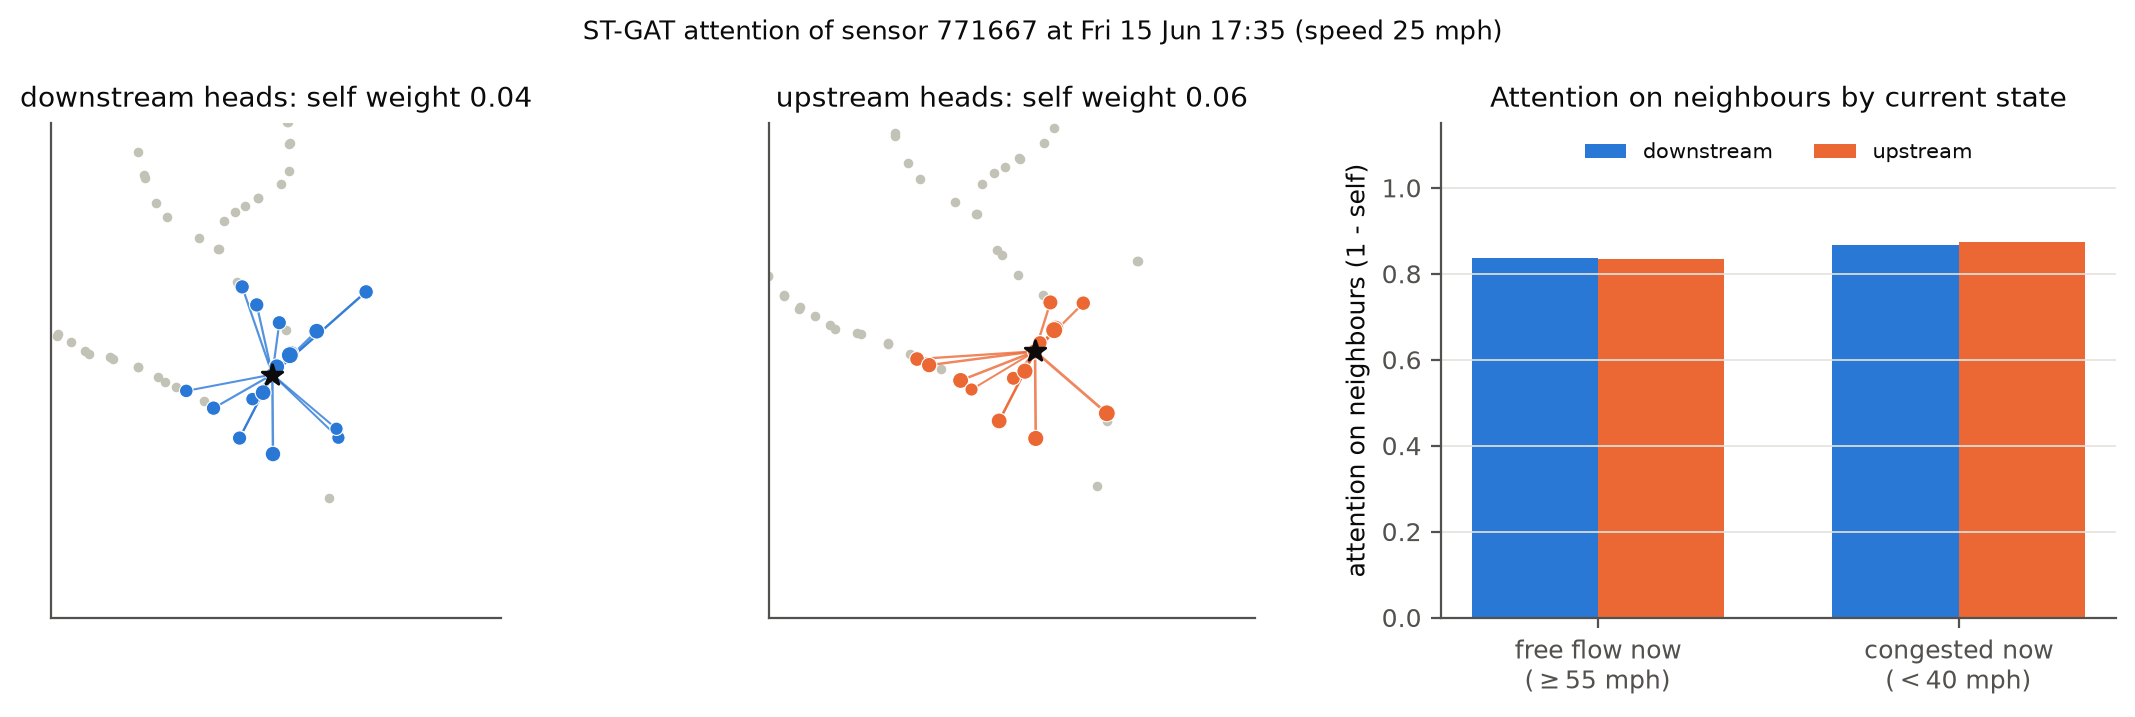
\includegraphics[width=0.95\textwidth]{p2_attention.png}\\[0.3em]
\small 84\,\% of attention goes to neighbours; slightly more when the sensor is congested
(0.84 $\to$ 0.87). Small shift: GAT attention is ``static'' (Brody et al.\ 2022), so we do not over-read it.
\end{frame}

\begin{frame}{Simulated signal-plan switching (offline only)}
\kicker{Optional deliverable \textperiodcentered{} no live-control claim}
\begin{columns}[T]
\column{0.42\textwidth}
\small
At each 5-min step, switch a sensor's upstream signal / ramp meter to a congestion plan if
speed in 15 min is expected $<$40 mph. Replay of the test period, 6,554 congestion onsets.
\vspace{0.6em}

\aside{METR-LA has no turning movements or timings, so we measure \emph{decision timing}, not delay. SUMO / CityFlow would be the next step.}
\column{0.55\textwidth}
\footnotesize\setlength{\tabcolsep}{3pt}
\begin{tabular}{lccc}
\toprule
Policy & Antic.\,\% & False\,\% & Switch/day \\
\midrule
Reactive (speed now) & 0.0 & 10.6 & 6.6 \\
XGBoost per segment & 19.8 & 7.7 & 4.1 \\
ST-GAT & 30.1 & 7.7 & \textbf{3.4} \\
Hybrid XGB$\to$GAT & \textbf{35.7} & \textbf{6.0} & 3.8 \\
\midrule
Oracle (true future) & 100 & 0.0 & 6.9 \\
\bottomrule
\end{tabular}\\[0.3em]
\aside{Antic.: plan already on 5--30 min before onset (median lead 10 min).}
\end{columns}
\end{frame}

\begin{frame}{Conclusions and limitations}
\begin{columns}[T]
\column{0.5\textwidth}
\kicker{What we showed}
\begin{itemize}\setlength\itemsep{0.4em}\small
\item Independent segment models have a measurable \hl{gap}: neighbour state predicts their errors.
\item Graph attention on the fixed road graph closes it: \hl{$-5\,\%$} MAE, $-6\,\%$ at peak, significant at all horizons.
\item Sound hybrid (cross-fitted, residual, zero-init) beats XGBoost; best at 15 min.
\item Masked outages: far more robust than 0-mph inputs.
\end{itemize}
\column{0.46\textwidth}
\kicker{Limitations \& next steps}
\begin{itemize}\setlength\itemsep{0.4em}\small
\item One seed per run; ablations on a shorter budget.
\item Speed only (no flow / occupancy); 4 months.
\item Window-shared, ``static'' attention $\to$ GATv2.
\item Offline signal replay $\to$ calibrated SUMO / CityFlow.
\end{itemize}
\end{columns}
\vspace{1em}
\centering\aside{Code, tests, report and app: project repository \textperiodcentered{} \texttt{streamlit run app/app.py}}
\end{frame}


\end{document}
